\documentclass{standalone}
\usepackage{tikz}
\usetikzlibrary{hobby, calc, intersections, spy, patterns}

\usepackage{pgfplots}
\usetikzlibrary{intersections, pgfplots.fillbetween}
% \pgfplotsset{compat=1.11}
% \usepgfplotslibrary{fillbetween}

\tikzset{%
  mark coordinate/.style={inner sep=0pt,outer sep=0pt,minimum size=1.2pt,
    fill=black,circle}%
}

\tikzset{%
  dots/.style args={#1per #2}{%
    line cap=round,
    dash pattern=on 0 off #2/#1
  }
}


\pgfdeclarelayer{bg}
\pgfsetlayers{bg,main}


\begin{document}
  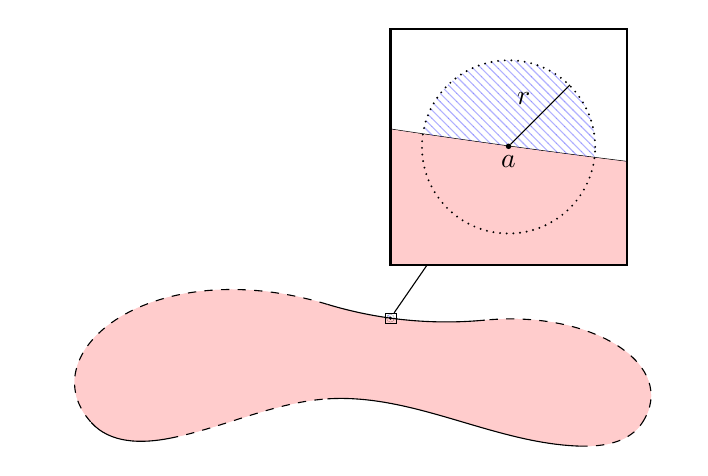
\begin{tikzpicture}[use Hobby shortcut]

    % This first draw creates the spy node; we draw twice so that the
    % line in the spy area can be thinner than it would be if we spied
    % directly on the end picture

    % This code is a hot mess
    \begin{scope}[spy scope, spy using outlines={rectangle,
      magnification=22, size=3cm, connect spies}]
      \begin{scope}[rotate=90, xshift=-6.5cm, yshift=-2.7cm]
        \draw[name path global=blobbdy, closed=true, line width=.025pt] ([blank=soft]6.5,-1) .. ([blank=soft]7.8,1) .. (8,3) .. ([blank=soft]6.5,6) .. (6.3,5) .. ([blank=soft]6.8,3) .. (6.2,-.2);
        \fill[red!20!white, closed=true] (6.5,-1) .. (7.8,1) .. (8,3) .. (6.5,6) .. (6.3,5) .. (6.8,3) .. (6.2,-.2);
      \end{scope}

      \coordinate (a) at (.5,1.325);
      \path[name path global=acircle] (a) circle (.05);
      \begin{scope}
        \clip (a) circle (1cm);
        \tikzfillbetween[of=blobbdy and acircle]{pattern=north west
            lines, pattern color=blue, opacity=0.3};
      \end{scope}

      \begin{scope}[rotate=90, xshift=-6.5cm, yshift=-2.7cm]
        \fill[red!20!white, closed=true] (6.5,-1) .. (7.8,1) .. (8,3) .. (6.5,6) .. (6.3,5) .. (6.8,3) .. (6.2,-.2);
      \end{scope}

      \draw[name path global=acircle, line width=.035pt, dots=260 per 1cm] (a) circle (.05);
      \spy on (a) in node at (2,3.5);
    \end{scope}

    \begin{scope}[rotate=90, xshift=-6.5cm, yshift=-2.7cm]
      \draw[closed=true] ([blank=soft]6.5,-1) .. ([blank=soft]7.8,1) .. (8,3) .. ([blank=soft]6.5,6) .. (6.3,5) .. ([blank=soft]6.8,3) .. (6.2,-.2);
      \draw[dashed, use previous Hobby path={invert soft blanks, disjoint}];
    \end{scope}

    \coordinate[mark coordinate] (a) at (a);
    % \draw[very thin, densely dotted] (a) circle (.17);

    \coordinate[inner sep=0pt, outer sep=0pt, minimum size=2pt,
    fill=black, circle] (ap) at (2,3.5075);


    \node[below] () at (ap) {$a$};
    % \draw[densely dotted] (ap) circle (1.2);
    \draw (ap) -- ($(ap) + (.78, .78)$) node[midway, above left] {$r$};

    % % Label below
    % \node (B) at (0,-1) {\huge $A$};



    % \draw

    % \draw

    % \node[below] () at (a) {$a$};

    % \spy on (65.0, 20.82) in node at (30, -50);

  \end{tikzpicture}
\end{document}
